\documentclass{article}
\usepackage[utf8]{inputenc}
\setlength{\parindent}{0pt} 
\usepackage{amssymb}
\usepackage{amsmath}
\usepackage{rotating}
\usepackage{graphicx}
\usepackage{subcaption}
\usepackage{mwe}
\usepackage{float}
\newcommand{\N}{\mathbb{N}}
\newcommand{\Z}{\mathbb{Z}}
\newcommand{\Q}{\mathbb{Q}}
\newcommand{\R}{\mathbb{R}}
\newcommand{\C}{\mathbb{C}}

\newcommand{\ra}{\longrightarrow}

\title{Final Part 1: Report}
\date{}
\author{Julian Lehrer}
\begin{document}
\maketitle
\textbf{Question 1a.} 

Using the singular value reconstruction with the $k \in \{ 20, 40, 80, 160, 320, 640, 1280, 2560, 3355\}$ largest singular values in the $\Sigma$ matrix, we obtain the following compressed images:

\begin{figure}[ht]
    \subfloat[$k=20$]{
      \begin{minipage}[c][1\width]{
         0.3\textwidth}
         \centering
         \includegraphics[scale=0.3]{images/compressed_20.png}
      \end{minipage}}
   \hfill 	
    \subfloat[$k=40$]{
      \begin{minipage}[c][1\width]{
         0.3\textwidth}
         \centering
         \includegraphics[scale=0.3]{images/compressed_40.png}
      \end{minipage}}
   \hfill	
    \subfloat[$k=80$]{
      \begin{minipage}[c][1\width]{
         0.3\textwidth}
         \centering
         \includegraphics[scale=0.3]{images/compressed_80.png}
      \end{minipage}}
\end{figure}

\vspace*{-20pt}
\begin{figure}[ht]
    \subfloat[$k=160$]{
      \begin{minipage}[c][1\width]{
         0.3\textwidth}
         \centering
         \includegraphics[scale=0.3]{images/compressed_160.png}
      \end{minipage}}
   \hfill 	
    \subfloat[$k=320$]{
      \begin{minipage}[c][1\width]{
         0.3\textwidth}
         \centering
         \includegraphics[scale=0.3]{images/compressed_320.png}
      \end{minipage}}
   \hfill	
    \subfloat[$k=640$]{
      \begin{minipage}[c][1\width]{
         0.3\textwidth}
         \centering
         \includegraphics[scale=0.3]{images/compressed_640.png}
      \end{minipage}}
\end{figure}

\vspace*{-20pt}
\begin{figure}[ht]
    \subfloat[$k=1280$]{
      \begin{minipage}[c][1\width]{
         0.3\textwidth}
         \centering
         \includegraphics[scale=0.3]{images/compressed_1280.png}
      \end{minipage}}
   \hfill 	
    \subfloat[$k=2560$]{
      \begin{minipage}[c][1\width]{
         0.3\textwidth}
         \centering
         \includegraphics[scale=0.3]{images/compressed_2560.png}
      \end{minipage}}
   \hfill	
    \subfloat[$k=3355$ (original image)]{
      \begin{minipage}[c][1\width]{
         0.3\textwidth}
         \centering
         \includegraphics[scale=0.3]{images/compressed_3355.png}
      \end{minipage}}
\end{figure}

With more values in the $\Sigma$ matrix of the SVD set to zero ($k=20$ being the fewest nonzero), the visual distortion is the highest. However, by just increasing $k=80$, the visual distortion is quite minimal, and for $k > 80$ I cannot see any visual difference with a small png. Now, defining the average Frobenius error of an $m \times n$ matrix $W$ by $\|W\|_F / (mn)$, we plot the errors of the difference between the original image and the $k$th SVD compression, i.e. $\|A-A_{k\sigma}\|_F/(mn)$.

\begin{figure}[H]
    \centering
    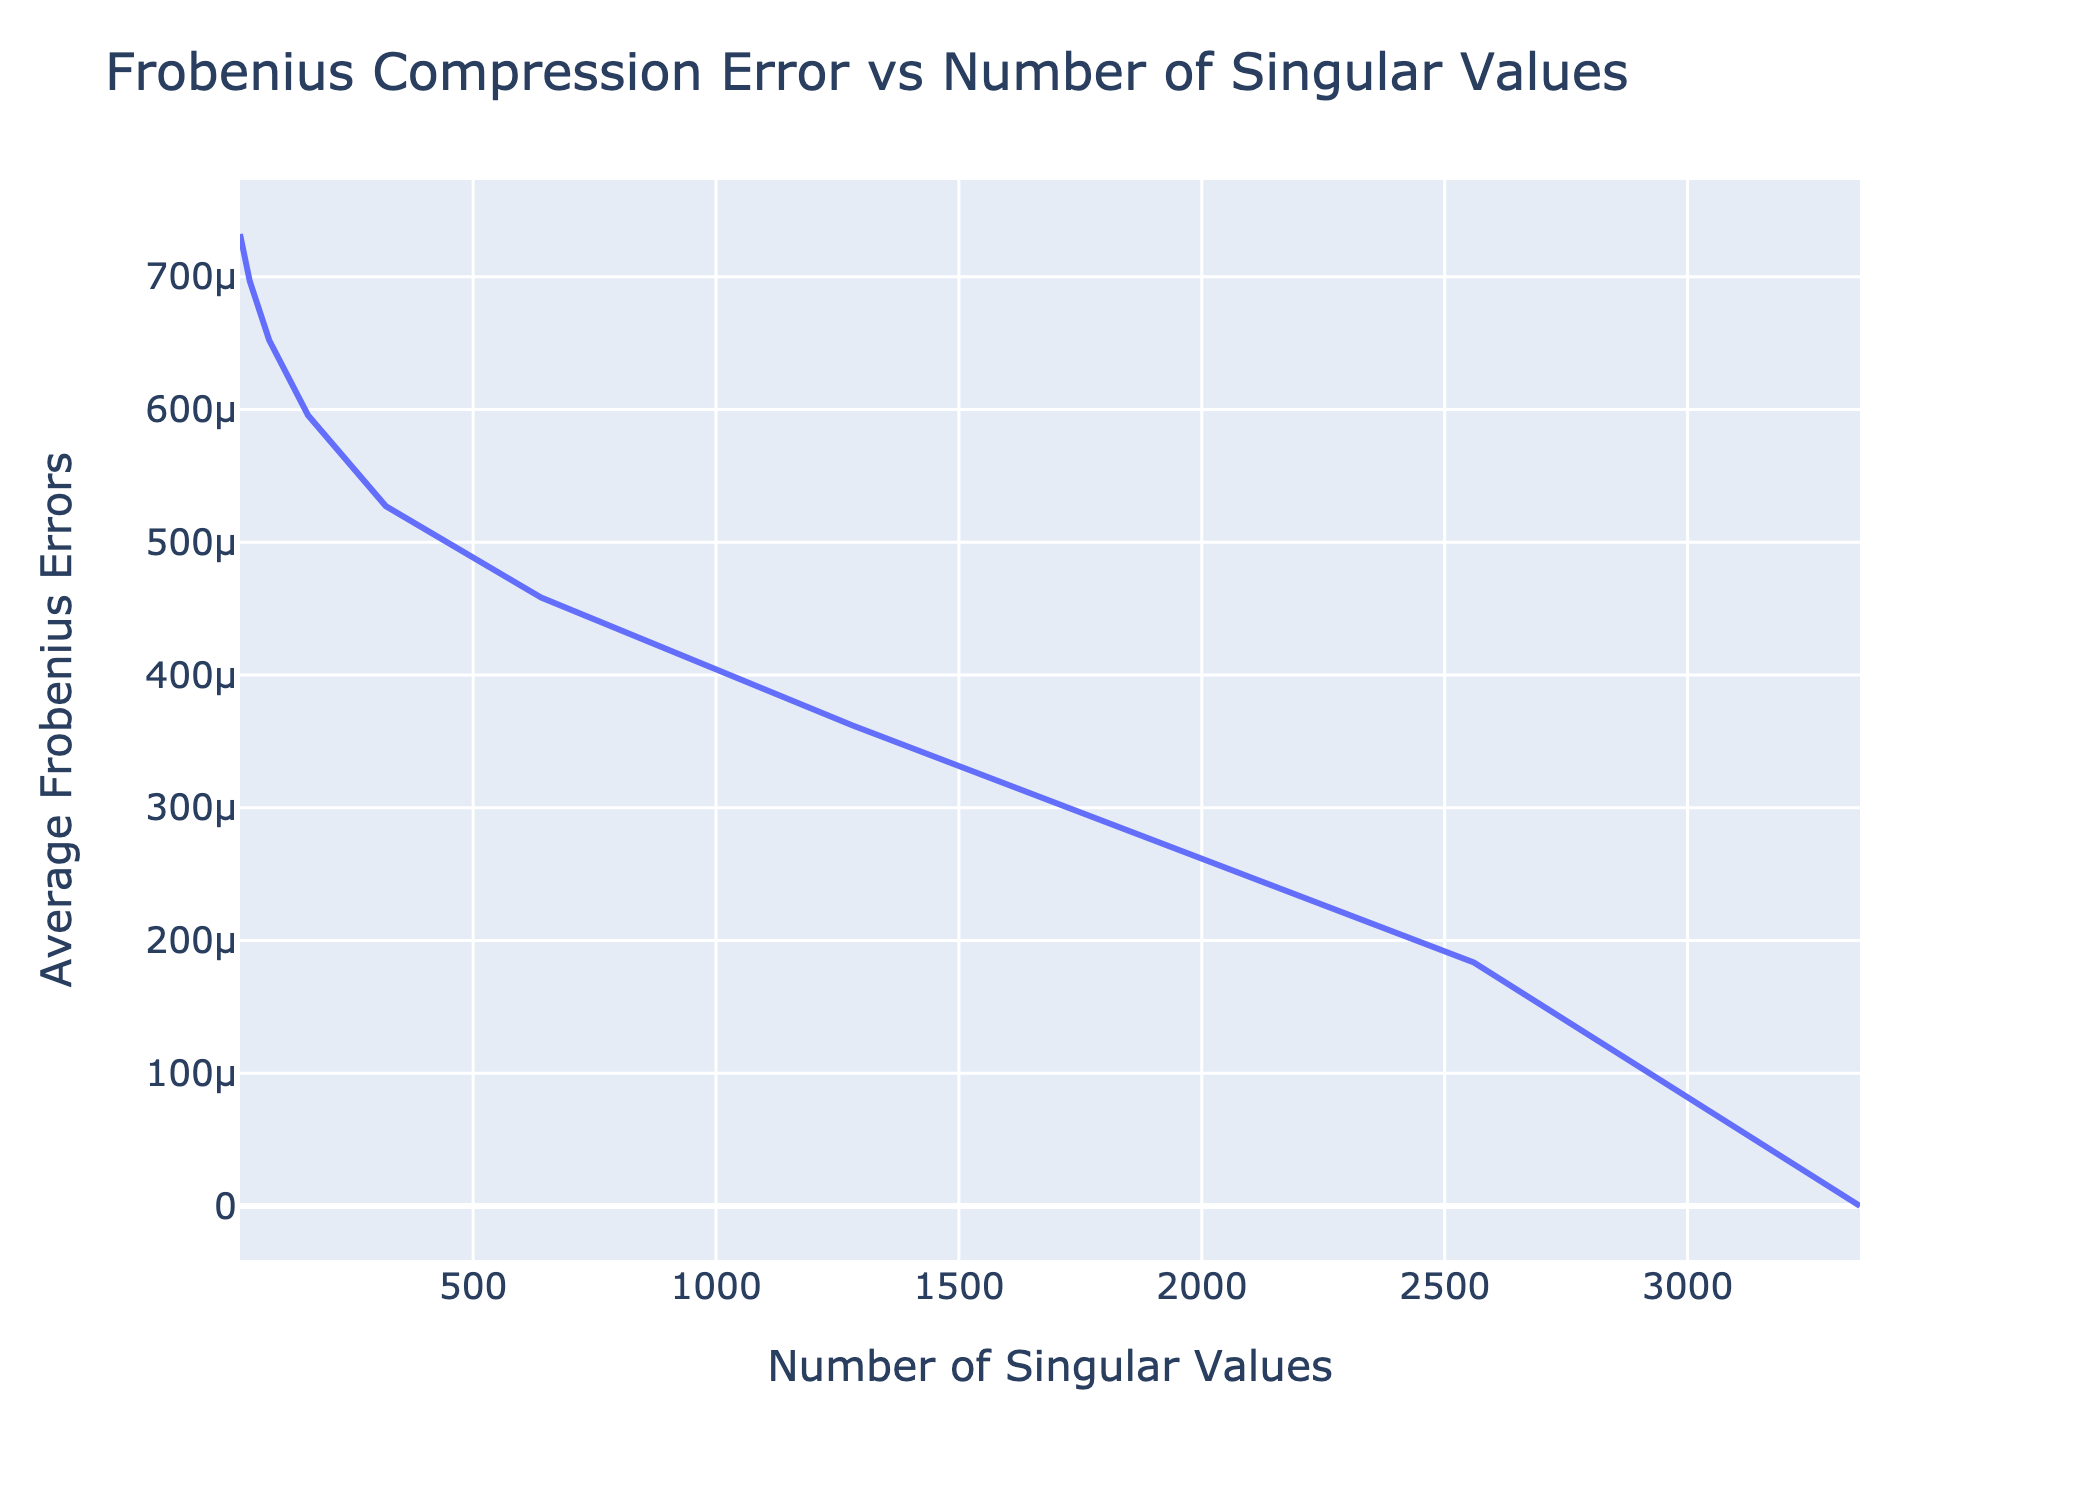
\includegraphics[scale=0.2]{images/errors.png}
\end{figure}

With $k=20$, we obtain an error less than $10^{-3}$, and for subsequent $k$ (with less distortion), we clearly do as well. \\

\textbf{Question b.1} 

The Gauss-Jacobi and Gauss-Seidel are both iterative methods for solving exact systems of equations of the form $Ax = b$, where $A$ is an $m \times m$ matrix and $b$ is an $m$-vector. For the former, we factorize $A=D+L+U$ where $D$ contains the diagonal elements and zeros elsewhere, and $L$ and $U$ contain the strictly lower and upper diagonal elements of $A$, respectively. Then we simply apply the iteration $x^{k+1} = D^{-1}\left(b-(L+U)x^{k}\right)$. \\

Note that for the Gauss-Jacobi method, the values $x_i^{k}$ obtained in the $k$th iteration remain completely unchanged until the $k+1$th iteration has been fully calculated. Instead, the Gauss-Seidel uses the values $x_i^{k+1}$ as soon as they're known. That is, once we calculate $x_{j}^k$ in the $j$th equation we use it in the $x_{j+1}^k$th equation. This difference allows us to only store one solution vector $x$, instead of having to store two for the current and previous. \\

For the Gauss-Jacobi method to converge, it is sufficient (but not necessary) that $A$ must be strictly diagonally dominant. More generally, we must have that $p(D^{-1}(L+U)) < 1$, that is, the spectrum is less than $1$. The Gauss-Seidel method is known to converge if $A$ is symmetric positive-definite, or if $A$ is strictly or irreducibly diagonally dominant. \\

In our case, we define a $10 \times 10$ matrix $A$ such that $a_{ij} = 1$ for $i \neq j$ and $a_{ii} = D$ for $D \in \{ 2,5,10,100,1000\}$. Below, visualize the convergence for the two methods, where $b_i = i$ for $i=1,...,10$. 

\begin{figure}[H]
  \centering
  % include first image
  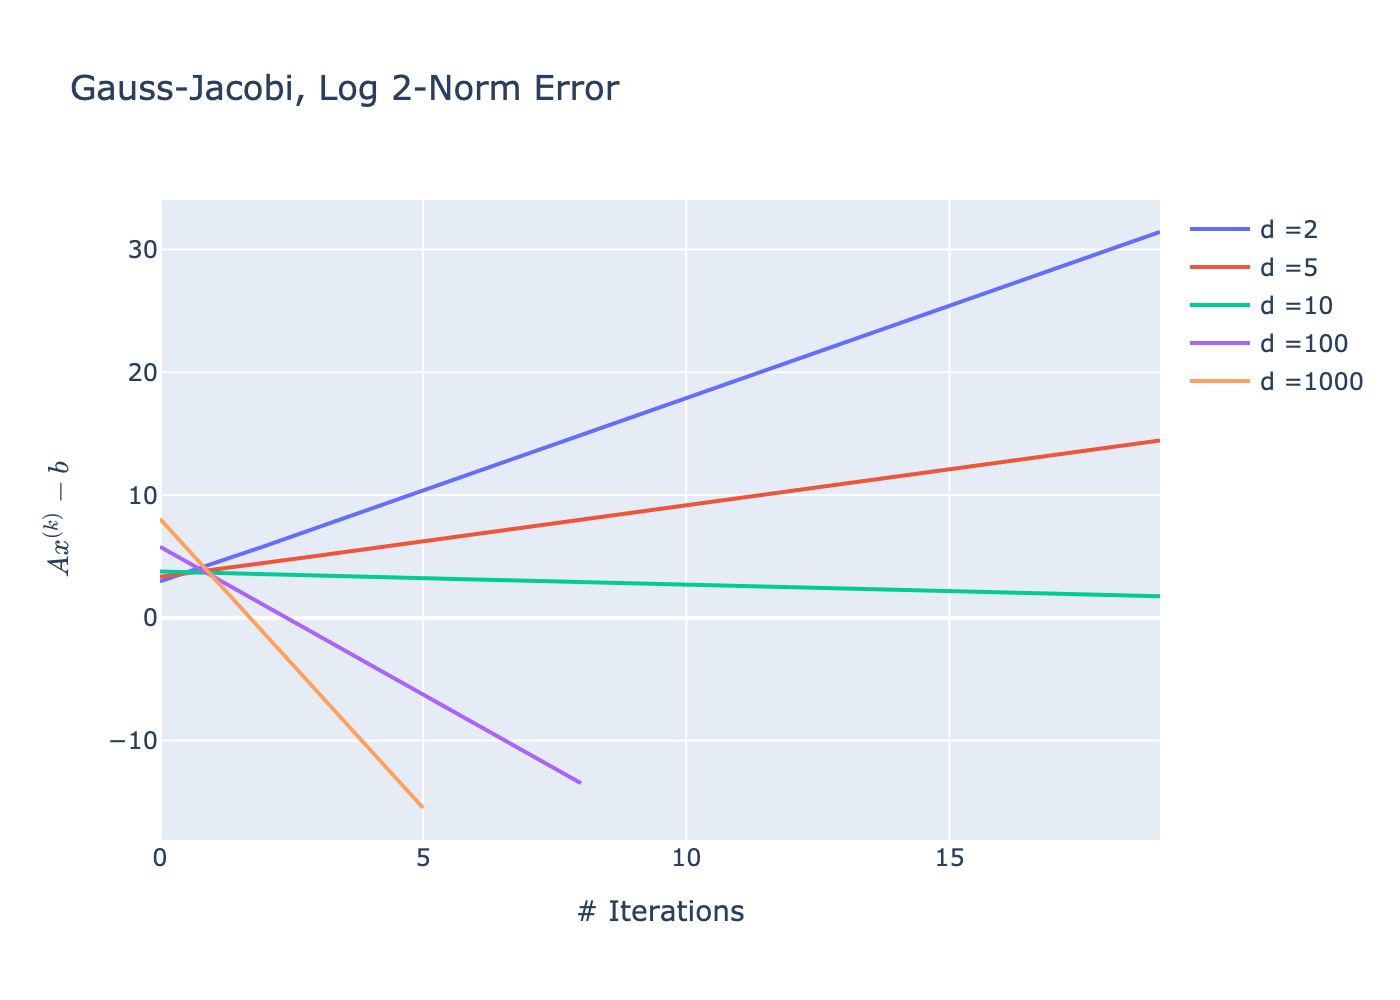
\includegraphics[width=\linewidth]{images/gauss_jacobi_error.png}  
  \caption{Convergence of Gauss-Jacobi, number of iterations vs log norm error.}
\end{figure}

\begin{figure}[H]
  \centering
  % include second image
  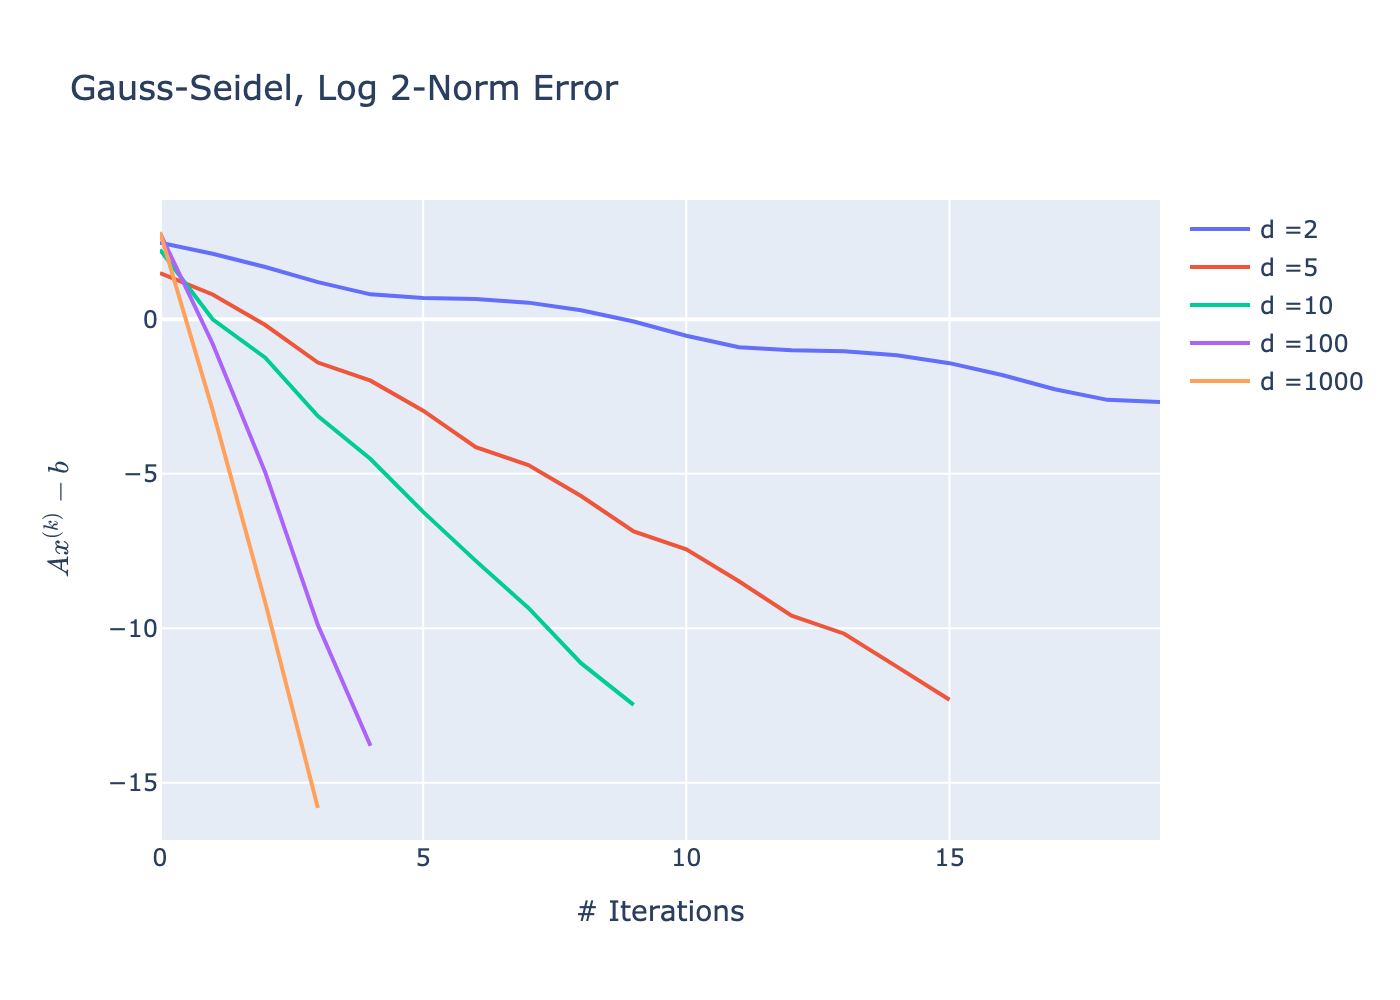
\includegraphics[width=\linewidth]{images/gauss_seidel_error.png}  
  \caption{Convergence of Gauss-Seidel, number of iterations vs log norm error}
\end{figure}

For the Jacobi method, we can see that for $D = 2,5$, the method diverges, wheres for the Gauss-Seidel method, these values converge (albiet quite slowly). For the Gauss-Seidel algorithm, since $a_{ii} = D$ and $a_{ij} = 1$, $i \neq j$, we have that $a_{ji}=a_{ij}$ for all $i$ and $j$. Therefore, $A$ is symmetric. Now, consider $\hat{x_i}$ to be the $i$th element of $x$ under the image of our matrix $A$. Then $\hat{x_i} = Dx_i+\sum_{j=1 \ j \neq i}^m x_j$. Therefore, $x_i \hat{x_i} = D(x_i)^2 +\sum_{j=1 \ j \neq i}^m x_jx_i$. For large enough $D$, this means $A$ is positive-definite, so the algorithm converges. \\

\textbf{Question b.2} 
The conjugate gradient algorithm numerically solves an exact system of equations $Ax = b$ where $A$ is symmetric and positive-definite. Then, this is equivalent to minimizing the function $f(x) = \frac{1}{2}x^T Ax-x^Tb$, since $\nabla f = Ax - b$ and solving $\nabla f = 0$ is equivalent to solving $Ax=b$. The conjugate gradient method therefore chooses $n$ conjugate directions, taking a step size towards the global minimum of $f$. The algorithm begins by choosing the direction like the gradient descent algorithm, i.e. opposite the direction of greatest ascent, or the gradient vector itself. So, $p_0 = b-Ax_0$. We then successively choose directions $p_k$ orthogonal to $p_{k-1}$, and search along our surface until we find the minima. \\

Here, we show the number of iterations convergence takes for the Gauss-Jacobi, Gauss-Seidel, and Conjugate-Gradient methods. 

\begin{center}
   \begin{tabular}{|c|c|c|c|}
      \hline
      D & Conjugate Gradient & Gauss-Jacobi & Gauss-Seidel\\
      \hline
      2 & 2 & Not reached & 58 \\ 
      \hline
      5 & 2 & Not reached & 16 \\ 
      \hline
      10 & 2 & 11 & 10 \\ 
      \hline
      100 & 2 & 11 & 5 \\
      \hline
      1000 & 2 & 11 & 4 \\
      \hline
   \end{tabular}
\end{center}

In general, the diagonal preconditioner is particularly efficient for diagonally dominant matrices. However, in the case of the conjugate gradient method, multiplying by the diagonal preconditioner given by $M = diag(\frac{1}{D},...,\frac{1}{D})$ means scaling each row by $\frac{1}{D}$, which in the case of our matrix is really just scaling the entire matrix down by a constant since the diagonals are constant. Therefore, we aren't actually changing the system in any way, and therefore the preconditioning isn't helpful at all. In the case where $A$ is a $10 \times 10$ matrix with $a_{ii} = i$, we have that the conjugate gradient algorithm converges in 10 iterations, and for $A$ being $100 \times 100$ with $a_{ii} = i$, it actually converges on the first iteration! This means that the initial vector $x$ given by $x=[1,...,1]^T$ (how I initialized $x_0$) was a particularly good guess in this case. \\
\end{document}
